\documentclass{scrreprt}
\usepackage{listings}
\usepackage{underscore}
\usepackage{graphicx}
\usepackage[bookmarks=true]{hyperref}
\usepackage[utf8]{inputenc}
\usepackage[english]{babel}
\hypersetup{
    bookmarks=false,    % show bookmarks bar?
    pdftitle={Software Requirement Specification},    % title
    pdfauthor={Jean-Philippe Eisenbarth},                     % author
    pdfsubject={TeX and LaTeX},                        % subject of the document
    pdfkeywords={TeX, LaTeX, graphics, images}, % list of keywords
    colorlinks=true,       % false: boxed links; true: colored links
    linkcolor=blue,       % color of internal links
    citecolor=black,       % color of links to bibliography
    filecolor=black,        % color of file links
    urlcolor=purple,        % color of external links
    linktoc=page            % only page is linked
}%
\def\myversion{1.0 }
\date{}
%\title
\usepackage{hyperref}
\begin{document}

\begin{flushright}
    \rule{16cm}{5pt}\vskip1cm
    \begin{bfseries}
        \Huge{SOFTWARE REQUIREMENTS\\ SPECIFICATION}\\
        \vspace{1.5cm}
        for\\
        \vspace{1.5cm}
        Hall Management Software\\
        \vspace{1.5cm}
        \LARGE{Version \myversion}\\
        \vspace{1.5cm}
        Prepared by : 1. Krish (21CS10037)\\
        2. Tanishq (21CS30054)\\
        3. Sourodeep (21CS00064)\\
        \vspace{1.5cm}
        \vspace{1.5cm}
        April 2, 2023\\
    \end{bfseries}
\end{flushright}

\tableofcontents

\chapter{Introduction}

\section{Purpose}
The purpose of this document is to describe the design of a web application that can handle the needs of the Hall Management Center of IIT Kharagpur by automating various book-keeping activities associated with the management of the different halls.
This is the first version of the application.
The application's scope covers an end-to-end system that is self-contained, possessing all the required interfaces and a corresponding backend for interacting with the system to achieve various management tasks.

\section{Document Conventions}
\textbf{Bold} text is used for software frameworks and tools.
\textit{Italicized} text is used for specific end-users of the application.
\section{Intended Audience and Reading Suggestions}
This SRS is for developers and testers who will be directly working on the implementation of the application. It is suggested that the reader familiarize themselves with the standard operating procedures of the halls in IIT KGP since this would help rationalize the various design decisions described in this document.

\section{Product Scope}
This software system will be a Hall Management System for our institute. This system will be
designed to streamline the process of everything related to the working of halls in our institute.
It will serve as a portal for the students, wardens, hall clerks and the HMC Chairman to access
information relevant to the respective parties.
More specifically, this system is designed to facilitate communication between the different
entities such as students and wardens, which would ensure smoother running of the halls and
provide an organised way to handle expenses and allocations.


\section{References}
IEEE. IEEE Std 830-1998 IEEE Recommended Practice for Software Requirements Specifications. IEEE
Computer Society, 1998.

\chapter{Overall Description}

\section{Product Perspective}
This application is needed to centralize the various book-keeping operations that are prone to errors and malicious failures. Manual management of these activities separately by the different halls in IIT KGP can lead to redundancies, lack of uniformity, etc. Students do not possess a simple mechanism to manage their interactions with their halls. For example, filing complaints would require the students to personally approach various individuals for resolution, sometimes with no accountability since there are no centralized complaint records available. Similarly, there are various such use cases that offer the potential for digitisation and the benefits associated with it. This document describes our vision for a web application that will handle all these situations in an accessible manner.
\section{Product Functions}
\begin{enumerate}
    \item Complaint resolution
    \item Fee management
    \item Grant management
    \item Expenditure control
    \item Staff management
\end{enumerate}
\section{User Classes and Characteristics}
The following user classes have been differentiated based on the subset of product features used. Each user class possesses a different interface into the application and are exposed to functions that are relevant to them.
\begin{enumerate}
  \item \textit{Mess managers}: Need to handle the dues, fees, and complaints relevant to the messes handled by them.
  \item \textit{Students}: Pay various fees and dues, register and view complaints.
  \item \textit{Hall clerks}: Manage the employment of temporary workers
  \item \textit{Wardens}: Handle complaints, manage payments to mess managers, handle financial grants from the HMC
  \item \textit{HMC chairman}: View various expenditures, allocation of grants to different halls 
  \item \textit{Administrators}: Manage student records and hall allocation
\end{enumerate}
\begin{figure}
    \centering
    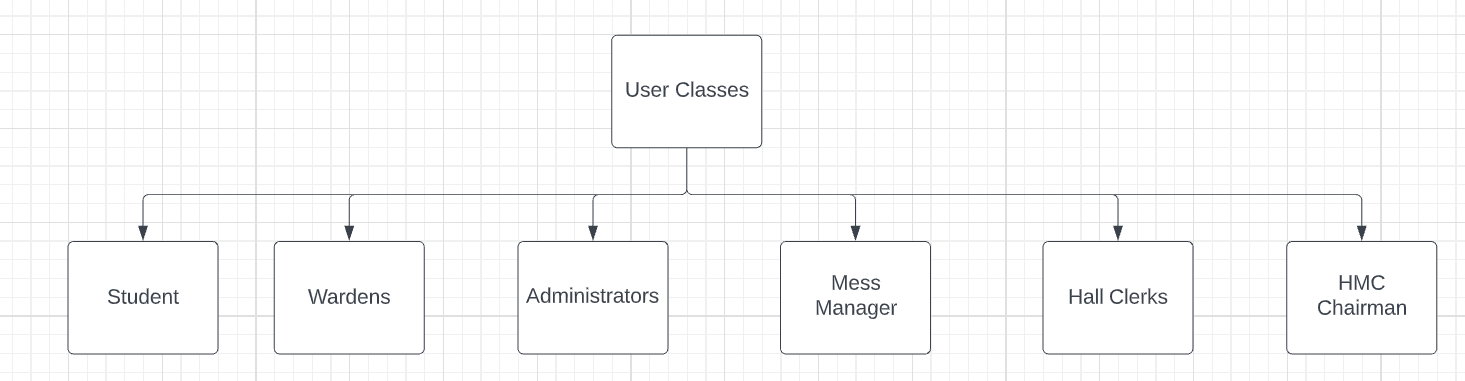
\includegraphics[scale=0.4]{classes.png}
    \caption{User classes}
    \label{fig:user_classes}
\end{figure}

\section{Operating Environment}
The application is designed to use the platform agnostic \textbf{Python} interpreter along with frameworks associated with it. The application server that handles incoming requests can be run on any platform that possesses a TCP/IP stack with support for \textbf{Django} and \textbf{Python}. The web application can therefore be run on \textbf{Windows Server} or \textbf{Linux}-based distributions which support the above tools.
The server should be connected to the local area network provided by the Computer and Informatics Centre in IIT KGP and should be appropriately configured to handle incoming requests. Any relevant firewall settings must be tweaked to allow high traffic to the server without dropping any requests.

\section{Design and Implementation Constraints}
Developers are limited to using Python for providing the backend services for the web application for the following reasons:
\begin{enumerate}
    \item Professors have enforced a rule necessitating the usage of either \textbf{C++}, \textbf{Java} or \textbf{Python}. This eliminates the possibility of writing the codebase with just \textbf{HTML}, \textbf{CSS} and \textbf{JavaScript} for the front-end combined with \textbf{JavaScript} on the backend (\textbf{Node.js}, etc.)
    \item \textbf{C++} and \textbf{Java} do not possess easy to use, batteries included frameworks like \textbf{Python}. The development time available for this project is less than three weeks. This necessitates the usage of pre-built mechanisms and libraries that Python possesses.

With these two constraints in mind, we have decided to use \textbf{Python} along with the \textbf{Django} framework for the web application.
\end{enumerate}
% \chapter{System Features}
% "IICT WEBSITE" is a result processing web software. So the main art of this product is to enter data of results and publish. 

\section{User Documentation}
The web application will possess a self-documenting, easy to use interface that does not require a specific set of manuals for any of the users. All the relevant information regarding the usage of the web application will be placed at the appropriate locations inside the different webpages and displayed when needed.


\section{Assumptions and Dependencies}
\begin{enumerate}
    \item The existence of a local network within the KGP campus. If this is absent, additional configuration would be required in terms of DNS, hosting, ISP handling, etc.
    \item End users should be able to connect to this network, otherwise access to the application will be limited to those with direct access to the servers. 
    \item The network should not have significant downtimes that can affect the utility of the application and its ability to handle incoming requests.
\end{enumerate}

\chapter{External Interface Requirements}

\section{User Interfaces}
\begin{figure}[h!]
    \centering
    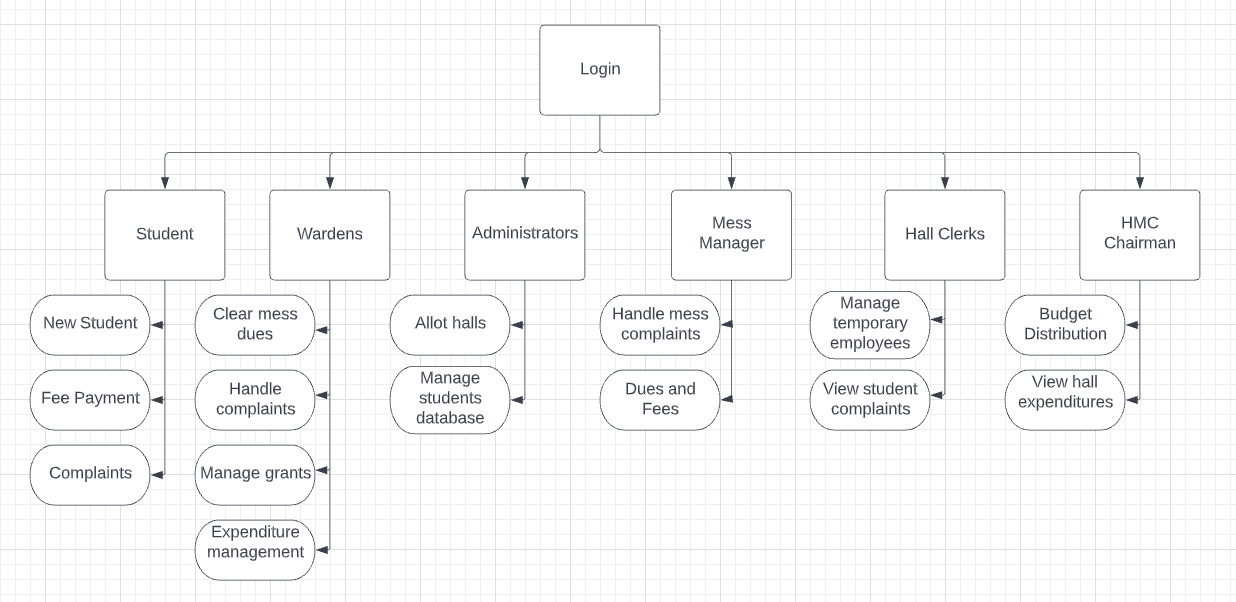
\includegraphics[scale=0.35]{user-interface.png}
    \caption{User interfaces}
    \label{fig:ui_diag}
\end{figure}

\section{Hardware Interfaces}
\begin{enumerate}
    \item The hardware used for this needs to be server computer with a processor fast enough to handle a large number of requests simultaneously. Preferably a multi-core system with distributed processes across the core will be suitable.
    \item Solid state drives instead of hard disks to boost the speed of information retrieval. Enables faster request handling.
    \item RAID systems to manage data redundancy. Ensures no user data is lost because of storage device failures by maintaining redundant copies as backup.
\end{enumerate}
\section{Software Interfaces}
\begin{enumerate}
    \item Web browsers needed on the end-users' systems to access the web application
    \item Graphical user interfaces combined with the browsers needed. Command-line interface won't be able to meaningfully handle the user interfaces provided in the web application.
\end{enumerate}
\section{Communications Interfaces}
\begin{enumerate}
    \item Will be using a standard TCP/IP stack available on most operating systems.
    \item Will use the \textbf{HTTPS} protocol to deliver webpages and handle user login
\end{enumerate}

\chapter{System Features}

\section{Complaint resolution system}
\subsection{Students}
\subsubsection{Description}
\begin{itemize}
    \item Mess related: A student can file complaints directly with the mess manager regarding food-related issues. 
    \item Hall related: Issues such as broken plumbing, absence of working electrical equipment, malfunctioning washing machines, etc., can be filed.
    \item Fees related: Any issues related to the payment of dues and fees can also be handled.
\end{itemize}
\subsubsection{Stimulus/Response Sequences}
\begin{itemize}
    \item Stimulus: Student wishes to file a new complaint.
    \item Response: Form is displayed where the student can enter the details of their complaint.
\end{itemize}
\begin{itemize}
    \item Stimulus: Student wants to review the action take report submitted by the warden or other authorities. 
    \item Response: System retrieves the report if submitted by the authorities via their portal and delivers it to the student.
\end{itemize}
\subsubsection{Functional Requirements}
\begin{itemize}
    \item \textbf{REQ1}: Digital forms for complaint registration
    \item \textbf{REQ2}: Tables for displaying complaint history
    \item \textbf{REQ3}: Webpage for displaying action take report
\end{itemize}

\subsection{Warden}
\subsubsection{Description}
The warden must be able to view all complaints registered by students and file action taken reports against them when necessary.
\subsubsection{Stimulus/Response Sequences}
\begin{itemize}
    \item Stimulus: Warden requests complaint history.
    \item Response: System uses its internal complaint database and returns the list of complaints.
\end{itemize}
\begin{itemize}
    \item Stimulus: Warden wishes to file an action taken report.
    \item Response: Form is displayed where the warden can enter the details and upload any relevant documents.
\end{itemize}

\subsubsection{Functional Requirements}
\begin{itemize}
    \item \textbf{REQ4}: Digital forms for the filing of action taken reports
    \item \textbf{REQ5}: Tables for displaying complaint history
\end{itemize}
Students will be able to view these complaints and the action taken reports filed by the warden. This enables transparency in the resolution process and helps in timely handling of issues.

\section{Hall Management}
\subsection{Hall clerks}
\subsubsection{Description}
The hall clerks must be able to add employees and register any petty expenses.
\subsubsection{Stimulus/Response Sequences}
\begin{itemize}
    \item Stimulus: Hall clerk wants to add new employee.
    \item Response: System brings up form for clerk to add the employee, asking for required details.
    \item Stimulus: Hall clerk wants to add new petty expense of the hall.
    \item Response: System brings up form for adding the new expense.
\end{itemize}

\subsubsection{Functional Requirements}
\begin{itemize}
    \item \textbf{REQ6}: Access of clerk to database of respective hall's employees.
\end{itemize}
\subsection{Temporary Employees' Salary Management}
\subsubsection{Description}
Hall clerks must be able to mark the days when temporary employees don't show up for work, and deduct pay accordingly. 
\subsubsection{Stimulus/Response Sequences}
\begin{itemize}
    \item Stimulus: Hall clerk wishes to mark a leave of absence when a certain temporary employee doesn't show up.
    \item Response: A webpage with a form is displayed that lets the clerk enter the relevant details.
\end{itemize}

\begin{itemize}
    \item Stimulus: Hall clerk requests the total amount payable to temporary employees.
    \item Response: A webpage with a form is displayed that lets the clerk enter the relevant details of the employees and returns the due amounts in an orderly fashion.
\end{itemize}
\subsubsection{Functional Requirements}
\begin{itemize}
    \item \textbf{REQ7}: Ability to track leaves of absence on a digital calendar.
    \item \textbf{REQ8}: Calculation of amount payable based on attendance
\end{itemize}


\begin{enumerate}
    \item Employee management of temporary employees such as gardeners, etc. and their payments.
\end{enumerate}



\section{Fees and dues management}
\subsubsection{Description}
Mess managers need to collect money from the students for food. Halls charge rents from their boarders. Apart from this, halls involve various other fees and costs. All these fees need to be recorded on a per-student basis and collected without irregularities.
\subsubsection{Stimulus/Response Sequences}
\begin{itemize}
    \item Stimulus: Mess manager wishes to enter a due amount against a certain student
    \item Response: A webpage with a form is displayed that lets the manager enter the relevant details.
\end{itemize}

\begin{itemize}
    \item Stimulus: Student requests the total amount owed with different filters (such as mess, rent, common room fees, etc).
    \item Response: A webpage with the relevant information is displayed.
\end{itemize}

\begin{itemize}
    \item Stimulus: Warden wishes to set the various fees associated with their hall such as rent.
    \item Response: A form is presented where the relevant information is collected and the internal database is updated to reflect the change.
\end{itemize}
\subsubsection{Functional Requirements}
\begin{itemize}
    \item \textbf{REQ9}: Ability to track the dues owed by different students.
    \item \textbf{REQ10}: Portal for mess managers to record the amount owed to them by each student.
    \item \textbf{REQ11}: Ability to set rent, etc, by wardens.
\end{itemize}


\section{HMC Employee Management}
\subsection{Description}
The employees working in the HMC will be registered with the web application. The payroll associated with the HMC will be handled. Salaries will be computed on a monthly basis and cheques will be issued to the employees.
\subsection{Stimulus/Response Sequences}
\begin{itemize}
    \item Stimulus: Administrator wishes to register a new staff.
    \item Response: A form that allows the admin to enter the details is displayed. The data is inserted into the database, and computations for their salary is started.
\end{itemize}

\begin{itemize}
    \item Stimulus: Administrator requests the total amount payable to a certain employee
    \item Response: A form is displayed after which the relevant information is displayed based on the input.
\end{itemize}
\subsubsection{Functional Requirements}
\begin{itemize}
    \item \textbf{REQ12}: Ability to track, add and delete registered employees.
    \item \textbf{REQ13}: Ability to view payments owed to different employees
\end{itemize}

\section{HMC Expenditure Management}
\subsection{Description}
\begin{itemize}
    \item HMC Chairman receives grant that is to be distributed to the various halls. This needs to be digitised.
    \item HMC incurs petty expenses such as repair works carried out, news paper and magazine subscriptions, etc. It should be possible to handle these expenses through the application.
\end{itemize}
\subsection{Stimulus/Response Sequences}
\begin{itemize}
    \item Stimulus: HMC Administrator wishes to enter a new petty expense.
    \item Response: A form that allows the admin to enter the details is displayed. The data is inserted into the database.
\end{itemize}

\begin{itemize}
    \item Stimulus: Warden wishes to enter expenditures against grants.
    \item Response: A form that allows the warden to enter the details is displayed. The data is inserted into the database and is shown to the HMC chairman when requested.
\end{itemize}

\begin{itemize}
    \item Stimulus: Administrator requests the petty expense report for a certain duration.
    \item Response: A form is displayed after which the relevant information is displayed based on the input after accessing the internal database.
\end{itemize}
\subsubsection{Functional Requirements}
\begin{itemize}
    \item \textbf{REQ13}: Ability to record petty expenses.
    \item \textbf{REQ14}: Ability to view expense reports on a timely basis.
    \item \textbf{REQ15}: Wardens should be able to enter expenditures against grants.
\end{itemize}

\section{Hall Occupancy Management}
\subsection{Description}
Wardens need to view which rooms are occupied and who is occupying them. This information needs to be quickly retrieved without having to go through paper records. The application helps them do that digitally.
\subsection{Stimulus/Response Sequences}
\begin{itemize}
    \item Stimulus: Warden requests an occupancy report.
    \item Response: A form that allows the admin to apply various filters is displayed. Based on the form input, the database is filtered and the relevant information is presented, such as number of rooms occupied.
\end{itemize}

\begin{itemize}
    \item Stimulus: Warden wishes to see who is occupying a certain room
    \item Response: A form is displayed after which the relevant information is displayed based on the input after accessing the internal database.
\end{itemize}
\subsubsection{Functional Requirements}
\begin{itemize}
    \item \textbf{REQ16}: Ability to see who is occupying a certain room
    \item \textbf{REQ17}: Ability to view an occupancy report.
\end{itemize}

% ---- expense report  ---- %
\section{Hall Expense Report}
\subsection{Description}
Wardens need to view the cash flow and various expenses owed. This information needs to be quickly retrieved without having to go through paper records. Mess fees, rent, grants, etc, can be centralized in a single location for the warden to review.
\subsection{Stimulus/Response Sequences}
\begin{itemize}
    \item Stimulus: Warden requests various expenses.
    \item Response: A form that allows the warden to apply various filters is displayed. Based on the form input, the expenses database is filtered and the relevant information is presented, such as the amount of owed by students, amount owed to mess managers, etc.
\end{itemize}

\begin{itemize}
    \item Stimulus: Warden requests a full accounting report
    \item Response: The system produces a table with all the expenses and payments accounted for. Cheques will automatically be generated. Warden will be able to print this report and the generated cheques.
\end{itemize}
\subsubsection{Functional Requirements}
\begin{itemize}
    \item \textbf{REQ17}: Ability to generate accounting reports
    \item \textbf{REQ18}: Ability to generate cheques.
    \item \textbf{REQ19}: Ability to submit the generated reports for audit.
\end{itemize}

\chapter{Other Nonfunctional Requirements}

\section{Performance Requirements}
\subsection{Server Up-time}
The system needs to keep running for long periods of time for accessibility so the hardware needs to be capable of that. Moreover the maintenance frequency needs to be low to have a stable experience for the end users.\subsection{Response Time}
The system needs to have a good response time as it will be repetitively used by various stakeholders in the Institute and the response time needs to keep up with the incoming requests. At the same time less used tasks like printing bills at the end of the month can be a little slow since they will be accessed much less frequently.
\subsection{System Dependability}
It determines the failure rate of the system, that is, the cases when the system receives an incorrect input or there is a random failure. The end user needs to be notified in such a scenario.
\subsection{Prominent Documents}
Since the system is also being used to maintain cash receipts and expenditure through the halls and generate official documents for the students' stay in their halls, the output needs to be clear, concise and consistent in a .pdf or another similar printable format.



\section{Safety Requirements}
There needs to be a regular audit to the cash flow through the hall since there is no check for the information entered by the mess manager. Moreover, audit also needs to be done for the budget distribution as there might be cases for fraud in the long run if left unchecked since the system is not verifying the data in any manner.

\section{Security Requirements}
\subsection{Secure Login}
The system should be protected against forced and malicious login attempts to access the software. The web interface needs to be continuously patched to fix bugs as and when they crop up.
\subsection{Verifiable Access}
The system is designed to serve multiple parties and their levels of access and their permissions are decided by their login IDs. Thus, the login and access to functionality should be robust and extremely secure since the system also deals with the finances of the institute.
\subsection{Student Information Must be Secure}
All the personal student information stored by the system should be safe and secure.

\section{Software Quality Attributes}
\subsection{Reliability}
The system must be dependable, which means it must constantly perform as expected with very low downtime and rate of failure. In absence of this the HCM will not be able to function smoothly.
\subsection{Information Accessibility}
To save the login credentials and the myriad types of data that the software uses, the application should be able to save, access and alter files on the system so that the information is retained even on successive runs.
\subsection{Maintainability}
The program should be easy to modify and add features to. The code should be clearly commented and the features well documented to allow for easy maintenance. The frameworks used should be well supported by their developers well into the future.

\end{document}